\RequirePackage{shellesc}
\documentclass[a4paper]{article}
\usepackage[document]{ragged2e}
\usepackage{fontspec}
\usepackage{geometry}
\usepackage{titlesec}
\usepackage{graphicx}
\usepackage{float}
\usepackage{minted}
\usepackage{enumitem}
\usepackage{indentfirst}
\usepackage[Export]{adjustbox} % Used to constrain images to a maximum size
\usepackage[font=large]{caption}
\geometry{left=2cm}
\geometry{right=2cm}
\geometry{top=2cm}
\geometry{bottom=2cm}
\setmainfont{Liberation Serif}
\setmonofont[Scale=0.7]{Hack}
\titlelabel{\thetitle. }
\renewcommand{\tablename}{Таблица}
\renewcommand{\figurename}{Рисунок}
\counterwithin{table}{section}
\counterwithin{figure}{section}
\captionsetup{justification=raggedright,singlelinecheck=false}
\renewcommand\large{\fontsize{14}{16}\selectfont}
\renewcommand{\theFancyVerbLine}{\textbf{\arabic{FancyVerbLine}}}
\sloppy

\setminted{
  linenos,
  breaklines,
  breakanywhere,
  breaksymbolleft=,
  fontsize=\fontsize{12}{12}\selectfont,
  numbersep=5pt,
}
\usemintedstyle{emacs}

\graphicspath{ {../4/pics/} }

\begin{document}
  \fontsize{14}{16}\selectfont

  \begin{titlepage}
    \begin{minipage}{0.2\textwidth}
      
\includegraphics[scale=0.4]{logo}
    \end{minipage}
    \begin{minipage}{0.7\textwidth}\centering
      \fontsize{10}{12}\selectfont
      \textbf{
        Федеральное государственное бюджетное образовательное учреждение \\
        высшего профессионального образования \\
        «Московский государственный технический университет имени Н.Э. Баумана» \\
        (МГТУ им. Н.Э. Баумана)
      }
    \end{minipage}

    \vspace{5cm}
    \centering
    \fontsize{16}{20}\textbf{
      Лабораторная работа №6 \\
      по курсу «Методы машинного обучения» \\
    }

    \vspace{5cm}
    \begin{flushright}
    Выполнил \\
    студент группы ИУ5-22М \\
    XXXX \\
    \end{flushright}
    \vspace*{\fill}
    Москва, 2023
  \end{titlepage}

  \justifying
  \setlength{\parindent}{1.25cm}

  \section{Задание}
  \begin{itemize}
    \item На основе рассмотренных на лекции примеров реализуйте алгоритм DQN.
    \item В качестве среды можно использовать классические среды (в этом случае используется полносвязная архитектура нейронной сети).
    \item В качестве среды можно использовать игры Atari (в этом случае используется сверточная архитектура нейронной сети).
    \item В случае реализации среды на основе сверточной архитектуры нейронной сети +1 балл за экзамен.
  \end{itemize}

  \section{Текст программы}
  \inputminted{python}{6.py}
  \pagebreak

  \section{Экранные формы с примерами выполнения программы}
  \begin{figure}[H]
    \centering
    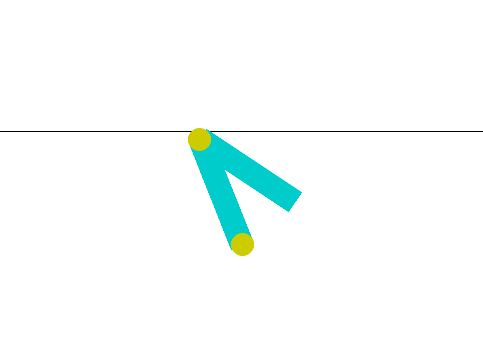
\includegraphics[scale=0.6]{61}
  \end{figure}
  \begin{figure}[H]
    \centering
    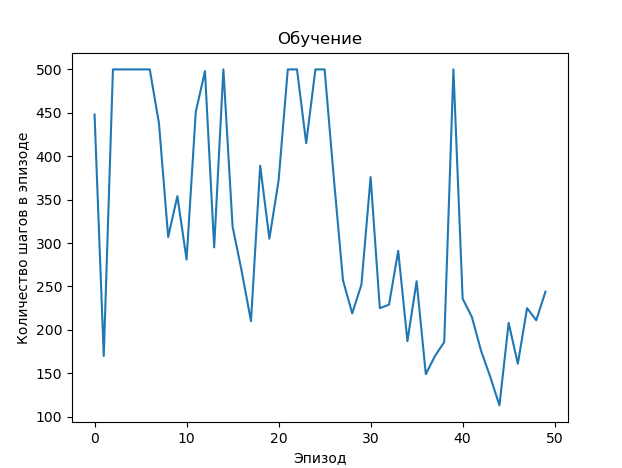
\includegraphics[scale=0.6]{62}
  \end{figure}
\end{document}
